\section{Exercise 1}

An application lets an employee edit the projects he is responsible for. 
A project has a name, a start and end date and a budget. 
The employee can create projects and assign other employees to them. 
Employees have a name, a code. Employees also have one or more skills. 
After logging in, the employee accesses a home page that displays:
\begin{itemize}
    \item The list of his projects, ordered by end date descending and with the list of employees allocated to each one. 
    \item The list of other employees, with the last name and the list of skills possessed. 
    \item A form for creating a project. 
    \item A form for choosing a project and assigning it to another employee. After creating a project or an assignment, the home page is displayed again, with the information updated. 
\end{itemize}
The entity relationship model is the following:
\begin{figure}[H]
    \centering
    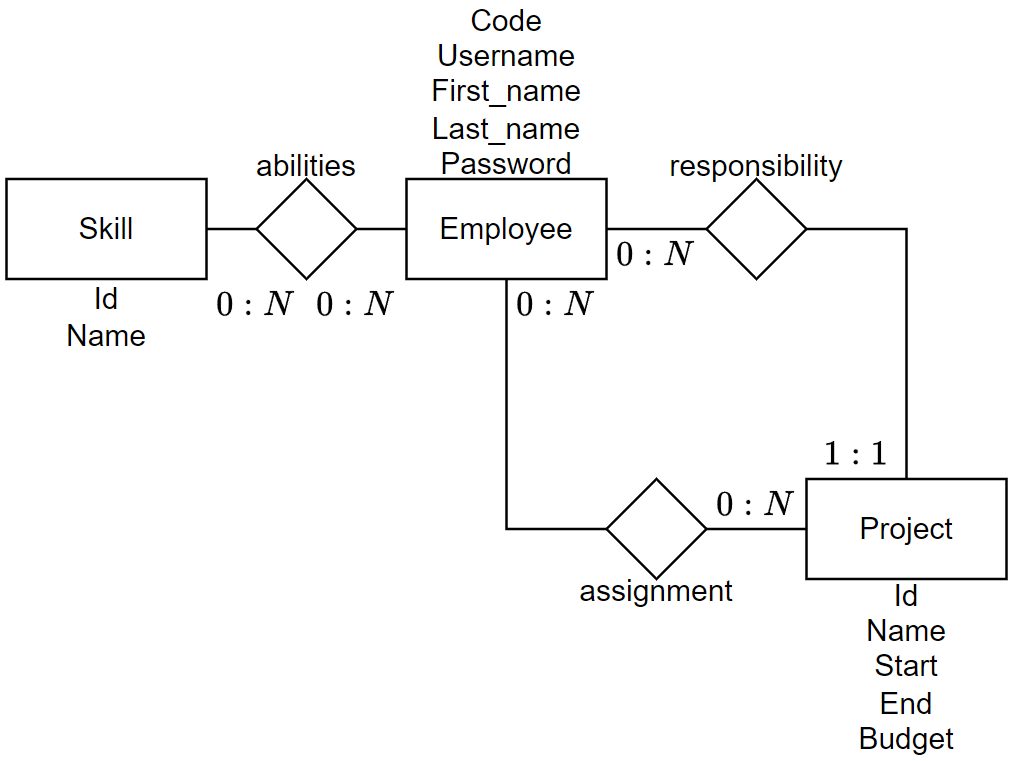
\includegraphics[width=1.0\linewidth]{images/e-r.png}
\end{figure}
The relational model is: 
\begin{itemize}
    \item Project(\underline{id}, name, start, end, budget, responsible)
    \item Emp$\_$prj(\underline{empid}, \underline{prjid})
    \item Employee(\underline{code}, firstname, lastname, username, pwd)
    \item Skill$\_$emp(\underline{skillid}, \underline{empid})
    \item Skill(\underline{id}, label)
\end{itemize}
Given the specifications write the entity classes of the ORM mapping, including annotations for the attributes and for the relationships, fetch type of attributes and of relationships, and operation cascading policies for relationships (when not by default). 

\subsection*{Solution}
We start by checking all the relationships in the E-R diagram: 
\begin{itemize}
    \item Responsibility: from employee to project we have to use the annotations: 
        \begin{lstlisting}[style=Java]
@OneToMany
@OrderBy("end DESC")
        \end{lstlisting}
        From project to employee we have to use these annotations: 
        \begin{lstlisting}[style=Java]
// This annotation can be omitted since it is implicit
@ManyToOne
        \end{lstlisting}
        The owner of the relation is entity project. 
    \item Assignment: from project to employee we have to use the annotations: 
        \begin{lstlisting}[style=Java]
@ManyToMany
// To let the client access the employees working in a project via relationship navigation
FetchType.EAGER
        \end{lstlisting}
        From employee to project we have to use these annotations: 
        \begin{lstlisting}[style=Java]
// This annotation can be omitted since it is implicit
@ManyToMany
        \end{lstlisting}
        The owner of the relation can be either project or employee. 
    \item Abilities: from employee to skill we have to use the annotations: 
        \begin{lstlisting}[style=Java]
@ManyToMany
        \end{lstlisting}
        From skill to employee we have to use these annotations: 
        \begin{lstlisting}[style=Java]
// This annotation can be omitted since it is implicit
@ManyToMany
        \end{lstlisting}
        The owner of the relation can be either skill or employee. 
\end{itemize}
We can now define the three entity mappings. The entity employee is defined as:  
\begin{lstlisting}[style=Java]
@Entity
public class Employee implements Serializable {
    ...
    @Id
    @GeneratedValue(strategy = GenerationType.IDENTITY)
    private int code;

    private String firstname;
    private String lastname;
    private String password;
    private String username;

    @ManyToMany(mappedBy = "employees", fetch = FetchType.EAGER)
    private List<Project> assignedProjects;

    @OneToMany(mappedBy = "manager", fetch = FeatchType.EAGER)
    @OrderBy("end DESC")
    private List<Project> managedProjects;

    @ManyToMany(mappedBy = "employees", fetch = FetchType.EAGER)
    private List<Skill> skills;
    ...
}
\end{lstlisting}
The entity project is defined as:  
\begin{lstlisting}[style=Java]
@Entity
public class Project implements Serializable {
    ...
    @Id
    @GeneratedValue(strategy=GenerationType.IDENTITY)
    private int id;

    private String name;
    private int budget;

    @Temporal(TemporalType.DATE)
    private Date start;

    @Temporal(TemporalType.DATE)
    private Date end;

    @ManyToMany(fetch = FetchType.EAGER)
    @JoinTable(name="emp_prj",
               joinColumns={@JoinColumn(name="projid")}, 
               inverseJoinColumns={@JoinColumn(name="empid")})
    private List<Employee> employees;

    @ManyToOne
    @JoinColumn(name="responsible")
    private Employee manager;
    ...
}
\end{lstlisting}
The entity skill is defined as:  
\begin{lstlisting}[style=Java]
@Entity
public class Skill implements Serializable {
    ...
    private static final long serialVersionUID = 1L;
    @Id
    @GeneratedValue(strategy=GenerationType.IDENTITY)
    private int id;
    private String label;
    @ManyToMany
    @JoinTable(name="skill_emp",
               joinColumns={@JoinColumn(name="skillid")},
               inverseJoinColumns={@JoinColumn(name="empid")}
               )
    private List<Employee> employees;
    ... 
}
\end{lstlisting}